
\section{Release Notes}

ESMF v2.1 is a first usable release of the Earth System 
Modeling Framework.  While the ESMF still has much growing to do
over the coming years, we expect modelers to find in this release 
tools that benefit real codes.  You may choose to start with the
highest level of functionality in the framework, the software
for representing models as components and coupling them to other
models; or the lowest level, the toolkits for data communication,
I/O, logging, or calendar management.  Wherever you begin, we hope
that you find the ESMF useful, and look forward to hearing your
comments on any aspect of the software.
Section \ref{sec:Support} 
of this document includes instructions on submitting comments on 
ESMF to our development team.

\section{What is the Earth System Modeling Framework?}

The ESMF is a structured collection of software building blocks that 
can be used or customized to develop 
Earth system model components, and assemble them into applications.  
The simplest view of the ESMF is that it consists of an
{\bf infrastructure} of utilities and data structures for creating 
model components, and a {\bf superstructure} for coupling them.  
User code sits between these two layers, making calls to the infrastructure
libraries beneath it and being scheduled and synchronized by the 
superstructure above it.  The configuration resembles a sandwich, as
shown in Figure~\ref{fig:TheESMFwich}.

The ESMF architecture is scalable, flexible paradigm for building highly 
complex climate, weather, and related applications from components such
as atmospheric models, land models, and data assimilation systems.  The 
ESMF is not a single master application into which all components must fit; 
rather it is a way of developing components so that they can be used 
in many different user-written applications.  Model components that adopt 
ESMF are designed to be usable in different contexts without code 
modification, and may be
incorporated into other ESMF-based modeling systems within the Earth 
science community.  In addition to high-level organization, ESMF provides 
a set of robust, portable, performance optimized libraries for regridding, 
data transfers, I/O, time management, and other common modeling functions.  
ESMF users may choose to extensively rewrite their codes to take advantage 
of the ESMF infrastructure, or they may decide to simply wrap user-written 
components in ESMF interfaces in order to adopt the ESMF architecture and 
utilize framework coupling services.

\section{The ESMF Reference Manual for Fortran}

The ESMF provides both Fortran and C++ versions of its interfaces
for many methods.  This {\it ESMF Reference Manual} is a listing of 
ESMF standard interfaces for Fortran.\footnote{Since the audience for it is 
small, we have not yet prepared a comprehensive reference manual for C++.}  

Interfaces are grouped by class.  A class is an object-oriented software 
design construct that embodies 
a specific concept like a physical field.  Superstructure classes 
are listed first in this {\it Manual}, followed by infrastructure 
classes.

The major classes in the ESMF superstructure are Components, which 
typically represent
large pieces of functionality such as models, model couplers, and 
dynamics and physics packages; and States, which are the data structures
used to store the fields and other data Components require or can 
make available.  There are both data structures and utilities in the ESMF 
infrastructure; classes include Fields, collections of Fields on the 
same grid (called Bundles), Arrays, and utilities for communication,
decomposition, time management, and application configuration.

For how to get started with ESMF, see the 
\htmladdnormallink{{\it ESMF User's Guide}}{http://www.esmf.ucar.edu/esmf_docs/ESMF_usrdoc}.  This document includes installation instructions, an
overview of the whole framework, an extended example of a coupled code, 
and other useful information. 

\begin{center}
\begin{figure}
\caption{Schematic of the ESMF ``sandwich'' architecture. In this design the framework consists of two parts, an upper level
{\bf superstructure} layer and a lower-level {\bf infrastructure} layer. User code is sandwiched between these two layers.}
\label{fig:TheESMFwich}
\scalebox{1.0}{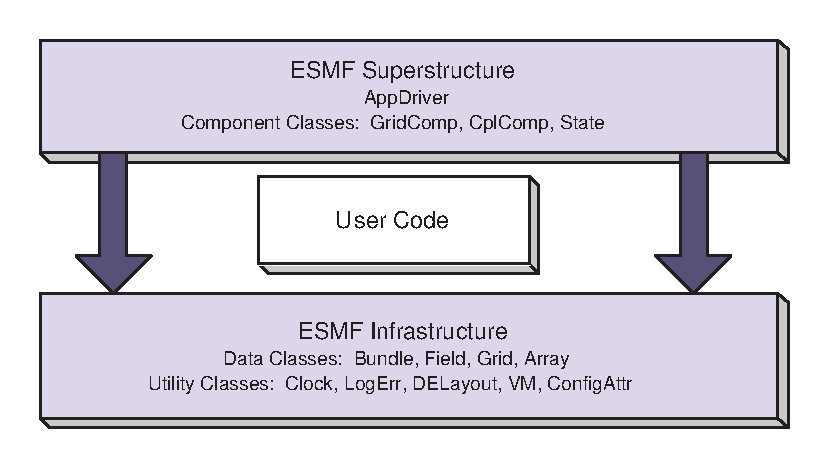
\includegraphics{ESMF_sandwich.eps}}
\end{figure}
\end{center}

